
\chapter{Evaluation}
\label{sec:Evaluation}
This chapter discribes and illustrates the experiments performed on the system. In the chapter, section \ref{sec:ExperimentsSetup} describes the experimental setup. Section \ref{sec:Datasets} describes the datasets used. Section \ref{sec:ResultsDetails} demonstrates and analyzes the results. 

The system has two main parts the DPSO stroke segmenation and symbol recogntion. Each part is evaluated sperately. The preprocessing procedures and computation is evaluated using their effect on the segmentation algorithm. These results are reported in section \ref{sec:ResultsDetails}. The effect of number of agents, the error thresholds and various other PSO paramters are investigated in Section \ref{sec:PSO}. %The results presented in Section \ref{sec:ResultsDetails} and \ref{sec:PSO}.  

The recognition system evalutation is presented in Section \ref{sec:SegmentationAlgorithms}. The recogntion rate (computed as the number of correctly recognized samples divided by the total number of samples in the test) for each segmentation algorithm compared to another segmenation algorithm are reported in \ref{sec:recognitionAlgorithms}. Next, a comparison between different shapes and datasets and it influence on the recogntion rate is presented in Section \ref{sec:EffectsofSymbolComplixity}. Finally, a  comparision between different feature vectors is reported in Section \ref{sec:featuresComparisions}.

\section{Datasets}
\label{sec:Datasets}
Two different data set were used, 
%For classifier and algorithm testing the system used a data set collected by
\begin{description}
	\item [Hse Dataset] (denoted as Hs-DB) Data set collected by \cite{HeloiseBeautification} and was previously used by \cite{Oltmans07} as benchmarck for sketch recognition problem. The data are drawn by 16 users each of them have drawn from 30 to 50 samples for each shape. Figure \ref{fig:symbolSet} shows the shapes used in the data set. The dataset was divided into training set and test set. Four different splits for the training and test data are generated from the dataset. In worth noting that \cite{HeloiseBeautification} and \cite{Oltmans07} achieved 96.7\% and  94.4\%  on this dataset respecitvily. %, 94.4\%  , which
%is comparable to the 96.7%  %The results displayed are the average recognition accuracy of the four splits resulted from the classifier after recognizing the symbols.
		\item [MultiDomain Dataset] (denoted as MD-DB) A dataset we collected manually from different users. The dataset contains symbols from three diffrent domains ( UML, mechanical and electrical engineering symbols). Data are collected from 4 different users each of them have drawn from 20 to 40 samples of each shapes. Figures \ref{fig:LogicSet} and \ref{fig:ElectSet} show some of the shapes used in the dataset. Symbols from different domains were gathered to evaluate the system thourhgtout different types of shapes. Useres were requested to draw symbols without any restriction on style,size or orientations. The dataset was divided into training set and test set. Four different splits for the training and test data are generated from the dataset. %The results displayed are the average recognition accuracy of the four splits resulted from the classifier after recognizing the symbols. 
\end{description}
 %We divided the dataset equally into training set and test set.  The results displayed are the recognition accuracy resulted from the classifier after recognizing the symbols. \\
%We divided the dataset into four sets each set contains four different users. Furthermore, each set is divided into train and test set where the trained set where used to train the classifiers and the test set where used for testing.  The algorithms are then tested using the four sets and the results are averaged.
\begin{figure}[]\centering
\fbox{  \parbox{8cm}{% 
		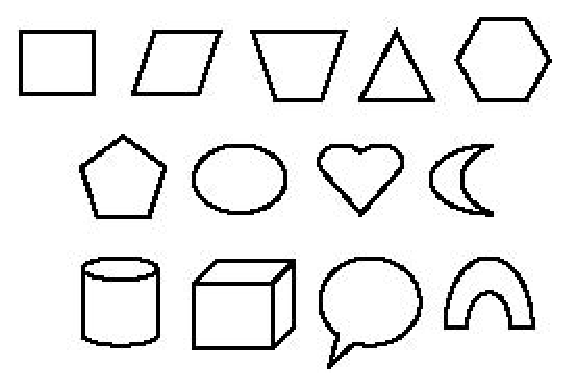
\includegraphics[scale=0.7]{images/symbolSet.eps}	}
		}
	\caption{The Symbol Set}
	\label{fig:symbolSet}
\end{figure}

\begin{figure}[]\centering
\fbox{  \parbox{6cm}{% 
		\includegraphics[scale=0.7]{images/logicSymbols.eps}	}
		}
	\caption{Example of Logic Symbols}
	\label{fig:LogicSet}
\end{figure}
\begin{figure}[]\centering
\fbox{  \parbox{8cm}{% 
		\includegraphics[scale=0.7]{images/SymbolsElectricalr.eps}	}
		}
	\caption{Example of Electrical Symbols}
	\label{fig:ElectSet}
\end{figure}



%\section{Evaluations techniques}
%\label{sec:EvaluationsTechniques}
%\section {Curvature estimation results}
%\label{sec:Curvatureestimationresults}
\section{Performance Measures }
\label{sec:PerformanceMeasures}

\begin{description}
	\item[Segmentation Error] The segmentation error is computed from each stroke after segmentation as computed from in $E_{alg}$ in Equation \ref{eq:bestFit2}. The error represents the sum of Square Root Error of the length from the point on the stroke to the estimated curve or line. 
	  
	\item [Recognition accuracy] We measure recognition performance for each algorithm by determining the number of correctly identified symbols in the whole dataset. Note that All the results are shown as the average of the four split of the dataset used. 
\end{description}

 

\section{Results}
\label{sec:ResultsDetails}

\subsection{PSO Algorithm}
\label{sec:PSO}

Figrue \ref{fig:SegErrPreCal} shows the \textit{Average Segmentation Error} using different preliminary calculation (Section \ref{sec:CurvatureCalculation}). The figure shows that using all computations (time difference, direction, speed and curvature) for each stroke decrease the Segmentation error. Figure \ref{fig:PossibledpPreCalculation} shows the average number of Possible dominant point $P_{pd}$ with respect to information used in the system. The results shows that the using all information increases the number of Possible dominate point $P_{pd}$ which in segmenation stage decreses the \textit{Segmenation Error}. It is worth noting that when using all information the number of Possible dominant point $P_{pd}$ is not the same as the sum of using every information alone. This is because we found out that there was some redundant points found using more than one information.  


   
\begin{figure}
	\centering
		\includegraphics[scale=0.5]{results/SegErrPreCal.eps}
	\caption{preliminary calculation effect}
	\label{fig:SegErrPreCal}
\end{figure}
 
 
\begin{figure}
	\centering
		\includegraphics[scale=0.5]{results/PossibledpPreCalculation.eps}
	\caption{Possible Dominant Point Count}
	\label{fig:PossibledpPreCalculation}
\end{figure}

	 	
 The effect of number of agents, the error thresholds and various other paramters was investigated. The result of these tests are shown in Figure \ref{fig:swarmtestingS1} and  \ref{fig:swarmtestingS2}. Figure \ref{fig:swarmtesting} shows that as the number of agents increases the \textit{Segmenation Error} value decrease. Simillar results for the maximum swarm iterations are shown in Figure \ref{fig:swarmtesting1} . Other algorithm parameters like $c_1$,$c_2$ that were mentioned in Section\ref{sec:ParticleSwarmAlgorithm} are tested using similar tests (Figure \ref{fig:swarmtesting} and \ref{fig:swarmtesting2}). The final values are for maximum number of iteration = 80 with 15 particles. The final number of agents and maximum swarm iteration used in the system was based trade off between error achieved versus the computation time. 
   
   
    
 \begin{figure}
	\centering		
	 \includegraphics[scale=0.3]{results/swarmalg1.eps}
	 	\caption{Segmentation Error Vs. Maximum iterations For ALgS1}
	 	\label{fig:swarmtestingS1}
	%\caption{Experiments results :} a)    b) c) 
\end{figure} 


    
 \begin{figure}
	\centering		
	 \includegraphics[scale=0.3]{results/swarmalg2.eps}
	 	\caption{Segmentation Error Vs. Maximum iterations For ALgS2}
	 	\label{fig:swarmtestingS2}
	%\caption{Experiments results :} a)    b) c) 
\end{figure} 


%The fig. \ref{fig:dataerrorvsiteration.jpg} display the effect of the size of swarm population on the number of vertex reported while segmenting the stroke.\footnote{The fewer the vertex the better the segmentation} The graphs shows that as the number of iteration increase there is a decrease in error until the error reach a saturation and any increase in number of iteration dose not affect the error calculated. Similar behavior is noticed in fig. \ref{fig:datapopulation.jpg}.  These curves and test result in choosing the swarm parameters $c_1,c_2$ and maximum number of iteration and the swarm population. The final values are for maximum number of iteration = 150 with 15 particle for better compensation in the time domain. 

%\begin{figure}
%	\centering
%		\includegraphics[scale=0.8]{images/dataerrorvsiteration.jpg.eps}
%	\caption{Error vs. iterations }
%	\label{fig:dataerrorvsiteration.jpg}
%\end{figure}
%\begin{figure}
%	\centering
%		\includegraphics[scale=0.8]{images/datapopulation.jpg.eps}
%	\caption{Swarm Population }
%	\label{fig:datapopulation.jpg}
%\end{figure}


\subsection{Segmentation Algorithms}
\label{sec:SegmentationAlgorithms}
The result of the segmentation algorithm can be viewed in the Figure \ref{fig:results1}. These result shows the originals stroke and the segmentation that the system generated for the stroke. The figure \ref{fig:results2} shows the result of \textsl{AlgS1} and \textsl{AlgS2} for the same input strokes.  Figure \ref{fig:results3} shows the ouptut of \textsl{Alg3} to the same set of input strokes. It clrearly shows that \textsl{AlgS2} have better segmentation results than both \textsl{AlgS1} and \textsl{Alg3} but since these segmentation are subjective to what the user intended to draw the next section will focus on the effect of the segmenation algorithm on the recognition accuracy. 

\begin{figure}

	\centering
				\subfigure{\includegraphics[scale=0.55]{results/result1.eps}}
					\subfigure{	\includegraphics[scale=0.6]{results/result1logic.eps}}
	\caption{Segmentation Results of \textsl{AlgS1}}
	\label{fig:results1}

\end{figure}

\begin{figure}
	\centering
			\subfigure{	\includegraphics[scale=0.55]{results/result2.eps}}
			\includegraphics[scale=0.6]{results/result2logic.eps}
	\caption{Segmentation Results of \textsl{AlgS2}}
	\label{fig:results2}
\end{figure}
\begin{figure}
	\centering
		\subfigure{
		\includegraphics[scale=0.55]{results/result3.eps}}
			\subfigure{\includegraphics[scale=0.55]{results/result3logic.eps}}
		
	\caption{Segmentation Results of \textsl{Alg3} }
	\label{fig:results3}
\end{figure}



\subsection {Recognition Algorithms}
\label{sec:RecognitionAlgorithms}


e performed several experiments to evaluate the presented recognition system. Firstly we tested recognition accuracy of shapes in the data set with both algorithms (\textsl{AlgS1} and \textsl{AlgS2}). We also implemented the segmentation algorithm described in \cite{earlyprocess} (\textsl{Alg3}) to use as reference to compare it with our swarm algorithms. Figure \ref{fig:test1} shows the accuracy achieved by each algorithm. The two swarm algorithms were tested with and without the ellipse fitting module. The ellipse detection module appears to be superior. The result shows that combining both  (\textsl{AlgS1} and \textsl{AlgS2}) out perform any single algorithm. %show that combining algoirthmsachieve higher accuracy than any single algoirthm. 
%improves the results.% with both the \textit{DPSO} algorithms.% The results show that both \textit{DPSO} algorithms achieve better result than other algorithms. 

 \begin{figure}
	\centering		
	 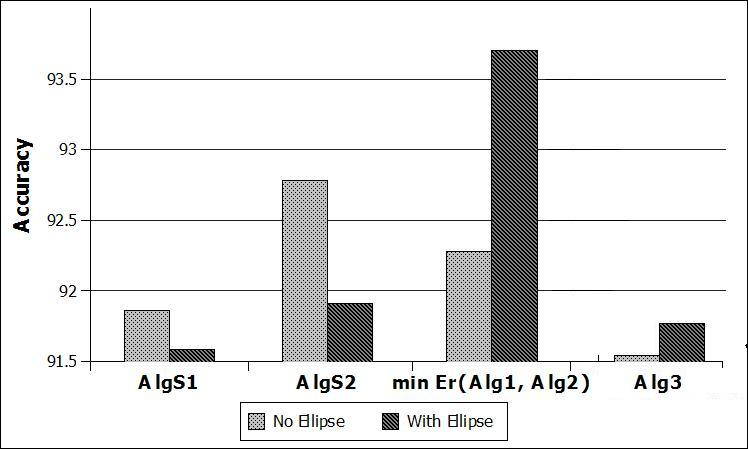
\includegraphics[scale=0.4]{results/testAlg.eps}
	 	\caption{Algorithm comparison} The recognition rate of different algorithms. 
	 	\label{fig:test1}
	%\caption{Experiments results :} a)    b) c) 
\end{figure} 


\subsubsection {Effects of Symbol Complixity }
 \label{sec:EffectsofSymbolComplixity}
 
 
\begin{figure*}
	\centering
		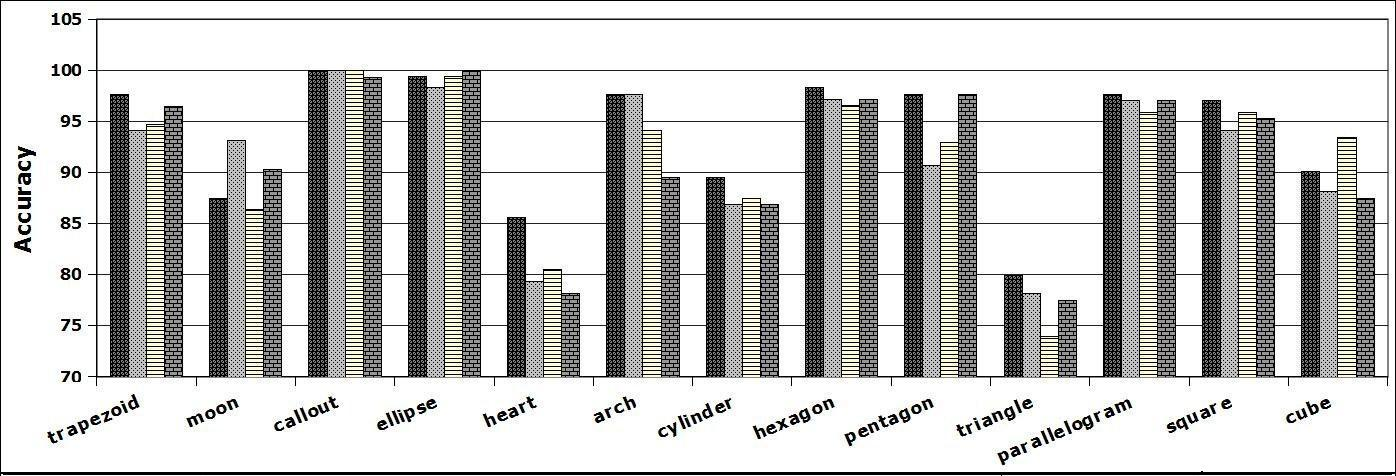
\includegraphics[scale=0.5]{results/testsym.eps}
	\caption{Symbols Comparison} The effect of symbol complexity.  %The graph shows the recognition rate of each symbol using different algorithms. 
	\label{fig:test2}
\end{figure*}  
The second experiment we implemented was to investigate the effect of symbol complexity and type on the recognition rate. Figure \ref{fig:test2} shows the achieved accuracy of each symbol by our algorithms compared to \cite{earlyprocess} (\textsl{Alg3}). It is clearly noted that symbols that have only line segments achieve higher accuracy rate than other symbols. The results indicate that algorithm \textsl{AlgS1} achieve better performance than algorithm \textsl{AlgS2} in the symbols that consist only of lines. This is understandable because algorithm \textsl{AlgS1} divides strokes into line segments only but \textsl{AlgS2} is able to divide strokes into lines and curves based on the minimum error of the segment itself. Algorithm \textsl{Alg3} gives good performance as long as the symbols consist of combination of lines and curves, if the stroke consists of only curve or lines the algorithm may lead to wrong segmentation result. This is because the system divides the stroke first to line segments then tries to decide if each segment can be represent better as a curve unlike algorithm \textsl{AlgS2} where the curve segments are tested while choosing the best segmentation. Combining both algorithm \textsl{AlgS1} and \textsl{AlgS2} improved the recognition rate of all symbols. The penalty for this improved performance is the computational time required to run both swarm algorithms. Table \ref{tab:ConfusionMatrix} shows the confusion matrix of symbols. The table shows that errors are only between two sets of symbols moon with triangles and trapezoid with triangles. This observation is understandable as the symbols are visually similar but the system must be able to differentiate between them. This lead us to the next experiment to choose best set of feature to recognize symbols. 
 \begin{table*}
	\centering
	%\small
%	\scalebox{0.7}{
		%	\begin{tabular}{|c|c|c|c|c|c|c|c|c|c|c|c|c|c|}\hline 
	\scalebox{0.7}{
		\begin{tabular}{|c|c|c|c|c|c|c|c|c|c|c|c|c|c|}\hline 
 Categories 	&ellipse	&heart	&trapezoid	&pentagon	&arch	&hexagon	&square	&triangle	&cube	&cylinder	&parallelogram	&moon	&callout\\ \hline
ellipse	&155	&9	&0	&0	&0	&5	&0	&0	&0	&0	&0	&6	&0\\ \hline
heart	&0	&109	&1	&1	&25	&0	&0	&1	&0	&0	&2	&1	&1\\ \hline
trapezoid	&0	&0	&103	&5	&2	&0	&0	&2	&0	&0	&34	&0	&0\\ \hline
pentagon	&0	&0	&20	&121	&0	&20	&6	&2	&0	&0	&1	&0	&0\\ \hline
arch	&0	&1	&13	&0	&86	&0	&0	&2	&3	&0	&2	&0	&0\\ \hline
hexagon	&0	&0	&0	&0	&0	&98	&0	&0	&0	&0	&0	&0	&0\\ \hline
square	&0	&0	&1	&0	&2	&0	&107	&14	&0	&0	&8	&1	&0\\ \hline
triangle	&0	&0	&7	&0	&1	&0	&0	&89	&0	&0	&12	&4	&0\\ \hline
cube	&0	&0	&0	&0	&0	&0	&0	&0	&147	&0	&0	&0	&0\\ \hline
cylinder	&0	&0	&0	&6	&2	&8	&16	&0	&4	&156	&1	&10	&0\\ \hline
parallelogram	&0	&0	&4	&0	&0	&0	&0	&0	&0	&0	&91	&0	&0\\ \hline
moon	&0	&3	&3	&2	&17	&0	&9	&17	&0	&0	&2	&133	&11\\ \hline
callout	&1	&34	&0	&22	&21	&22	&16	&25	&0	&0	&0	&0	&143\\ \hline
		\end{tabular}
			}
 		%\end{tabular}
 	%}
	\caption{Confusion Matrix}
	\label{tab:ConfusionMatrix}
	%\end{minipage}
\end{table*}
 
 
\subsubsection{Features Comparisions}
\label{sec:featuresComparisions}
Different feature sets are tested to determine the best features that can used in sketch and symbol recognition. Figure\ref{fig:testFeaturesAllHS} shows the result of different feature sets from the basic four sets (\textbf{FS1,FS2,FS3,FS4}). Result shows that (\textbf{FS2}) Rubine features \cite{gestureexample12} gives the worst results when used alone without any other features. This is because they are mainly computed for single stroke gestures and fare bad in multi-stroke symbols \cite{compareFeaturSVM}. Features \textbf{(FS4)} gives good results but it is improved by adding structural features \textbf{(FS1)}.  Figure \ref{fig:testFeaturesAllMD} shows the simillar results on \textsl{MD-DB} multidomain database. The figure shows that on this dataset \textbf{FS1} performe better than on \textsl{HS-DB}, this is a result that shapes in the \textsl{MD-DB} has more structural difference than shapes in \textsl{HS-DB}.
 \begin{figure}
	\centering
		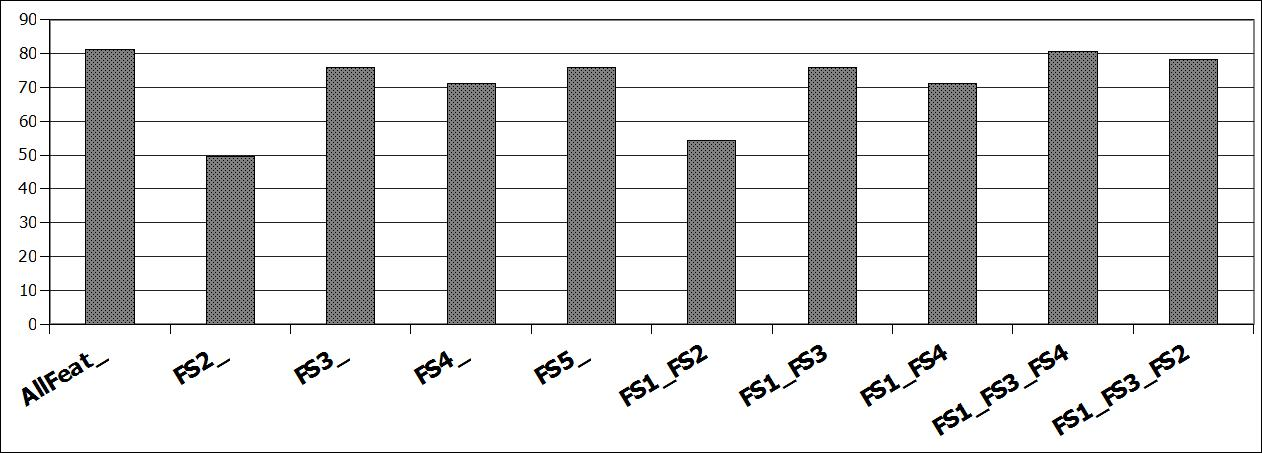
\includegraphics[scale=0.5]{results/testFeat.eps}
	\caption{Feature Comparison} The effect of different features on accuracy on \textsl{Hs-DB}.  %The graph shows the recognition rate of each symbol using different algorithms. 
	\label{fig:testFeaturesAllHS}
\end{figure}  

 \begin{figure}
	\centering
		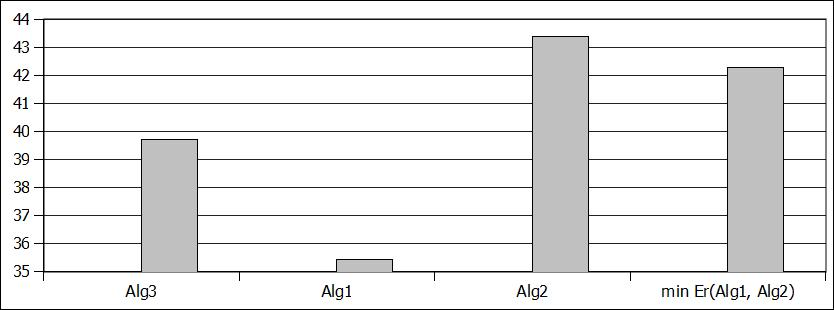
\includegraphics[scale=0.5]{results/testF1.eps}
	\caption{Feature Comparison} The effect of different features on accuracy on \textsl{MD-DB}.  %The graph shows the recognition rate of each symbol using different algorithms. 
	\label{fig:testFeaturesAllMD}
\end{figure}  


\section{Summary}
\label{sec:ResultSummary}

The result illustrated in this chapter shows the work done on the system and experiments performed. The results shows that the ellipse detection and PSO swarm algorithms gives better performance than other known systems. 

%\section{ BenchMark Results }
%\label{sec:BenchMarkResults}

